\section{Contrastando con la realidad}

Finalmente realizamos una serie de experimentos contra las IP's de las universidades seleccionadas, enviando un gran volumen de sucesivos ``pings'' con la finalidad de simular una conexión (y su consiguiente envío de paquetes) frente a dichas direcciones.

El envío de los pings lo hicimos por medio de un script realizado para dicha finalidad, implementado en Python y con las herramientas proporcionadas por Scapy. Por cada uno de los pings enviados (paquetes Echo Request de ICMP) se midió el tiempo requerido para obtener una respuesta (paquete Echo Reply de ICMP). Luego de realizarlos, se analizaron los resultados obtenidos, ya sea para las respuestas efectivas (la estimación del Round Trip Time correspondiente) y para los paquetes perdidos (para obtener una estimación de la probabilidad de pérdida de paquetes). 

El total de paquetes Echo Request enviados fue de 1000. Consideramos que sería un valor lo suficientemente grande como para tener una gran cantidad de mediciones válidas, sin ser un número que requiera demasiado tiempo de cómputo.

\subsection{Estimación de RTT con alfa fijo}

En primer lugar, para estimar los RTT de cada simulacro de conexión, analizamos las mediciones realizadas para los paquetes recibidos según la siguiente fórmula que involucra los diferentes valores obtenidos en el muestreo y un coeficiente \alpha que mantuvimos en el intervalo $[0..1]$:

\begin{center}
EstimatedRTT[i] = \alpha \texttimes EstimatedRTT[i-1] + (1 − \alpha) \texttimes SampleRTT[i]
\end{center}

Fuimos tomando algunos valores de alfa que consideramos representativos dentro del intervalo mencionado, y para cada valor seleccionado, realizamos la estimación con diversos subconjuntos de muestras RTT, cada vez de mayor volumen. Para el caso de 100 paquetes se tomaron las primeras 100 mediciones, luego las 200 primeras y así sucesivamente.

El gráfico siguiente revela las estimaciones obtenidas para el Round Trip Time relativo al experimento con la Universidad Humboldt de Berlín. Como mencionamos previamente, fijando diversos valores de alfa fuimos tomando cantidades cada vez mayores de muestras reales. Se puede apreciar notoriamente como a mayores valores del coeficiente alfa, la estimación es mas consistente y menos suceptible a las bruscas variaciones de la muestra original (algo que se observa en el caso \alpha = 0, donde EstimatedRTT[i] = SampleRTT[i] para todo valor de i).

\centerline{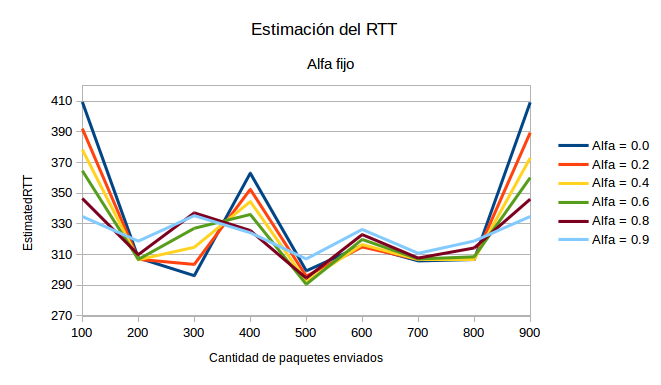
\includegraphics[width=0.8\textwidth]{imagenes/3ra_parte/ping_varios_alfa_fijo_variando_n_alemania.png}}

En el caso de la Universidad de Moscú, en general los valores fueron mas cercanos entre sí a pesar de incrementar la cantidad de paquetes a analizar. Pero al llegar a valores cercanos a los 900 paquetes, la estimación vuelve a crecer mas lentamente para valores de alfa mayores en comparación con los valores inferiores. 

Comenzamos a considerar que esto puede ser una tendencia real y que efectivamente las estimaciones con un alfa mas grande se normalizan mejor frente a un valor promedio en contraposición a las estimaciones que utilizan coeficientes alfa mucho menores, donde las mismas sufren de variaciones mucho mayores.

\centerline{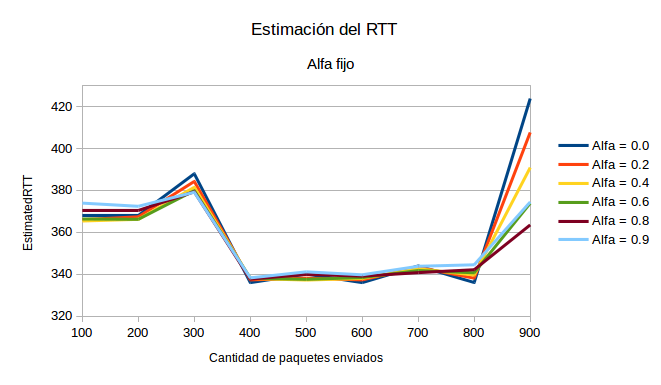
\includegraphics[width=0.8\textwidth]{imagenes/3ra_parte/ping_varios_alfa_fijo_variando_n_rusia.png}}

La Universidad de Tokio no es la excepción y vemos como ocurre nuevamente la misma situación. Sin importar la cantidad de paquetes ICMP enviados al host de la institución, las estimaciones hechas con valores de alfa superiores, son mucho mas estables entre sí con respecto a las estimaciones restantes.

\centerline{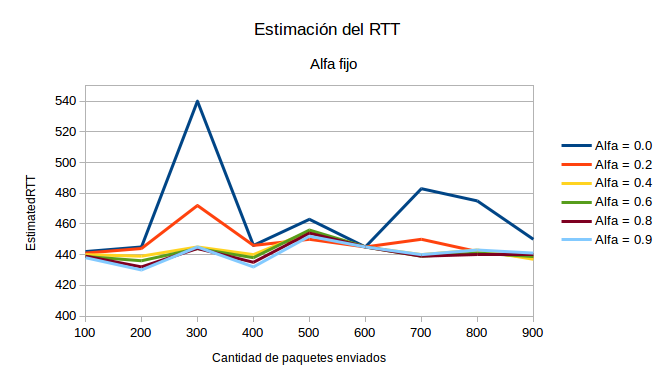
\includegraphics[width=0.8\textwidth]{imagenes/3ra_parte/ping_varios_alfa_fijo_variando_n_japon2.png}}

Finalmente, la Universidad de Boston refleja la situación que venimos remarcando de una manera aún mas clara. Se observa claramente como las estimaciones que utilizan el valor de alfa mas grande, son las mas estables a lo largo de los diferentes experimentos con las diversas cantidades de paquetes.

\centerline{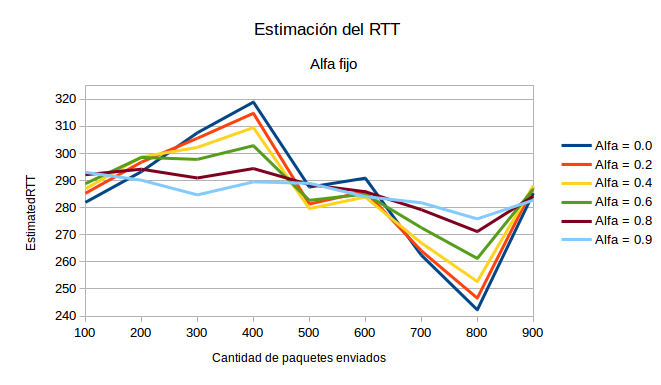
\includegraphics[width=0.8\textwidth]{imagenes/3ra_parte/ping_varios_alfa_fijo_variando_n_eeuu.png}}

\subsection{Estimación de RTT con cantidad fija de paquetes}

Ahora realizaremos una nueva serie de experimentos con las mismas muestras de RTT's obtenidas originalmente, pero esta vez fijaremos algunos subconjuntos con diferentes cantidades y veremos como van variando las estimaciones al incrementar el alfa para cada caso.

Para nuestra primer universidad, Humboldt de Berlín, observamos como en los tres casos al aumentar el coeficiente, todas las curvas tienden a un valor común, cercano a los 330. En aquellos casos donde las mediciones comenzaron por debajo de la estimación final, las estimaciones parciales fueron aumentando en tendencia a acercarse a dicho valor. En contrapartida, la curva que comenzó con mediciones superiores a la estimación final, terminó tendiendo a minimizar sus estimaciones parciales.

\centerline{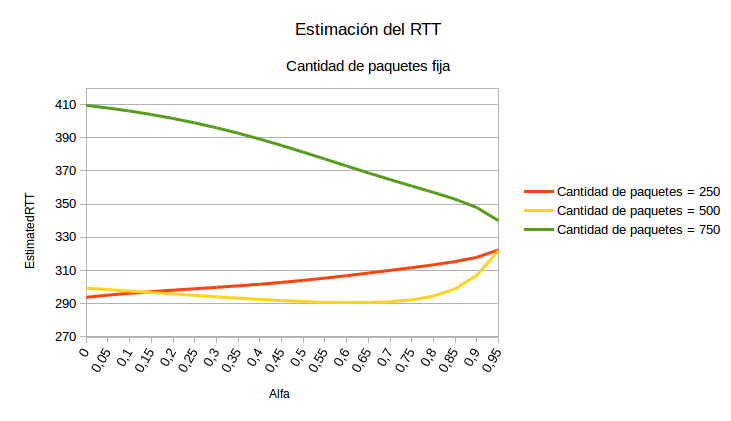
\includegraphics[width=0.8\textwidth]{imagenes/3ra_parte/ping_varios_n_fijo_variando_alfa_alemania.png}}

En el caso de la Universidad de Moscú, los valores se mantuvieron muy estables y cercanos entre sí, presentando una ligera aproximación de todas las curvas al final del experimento, al incrementar el valor de alfa.

\centerline{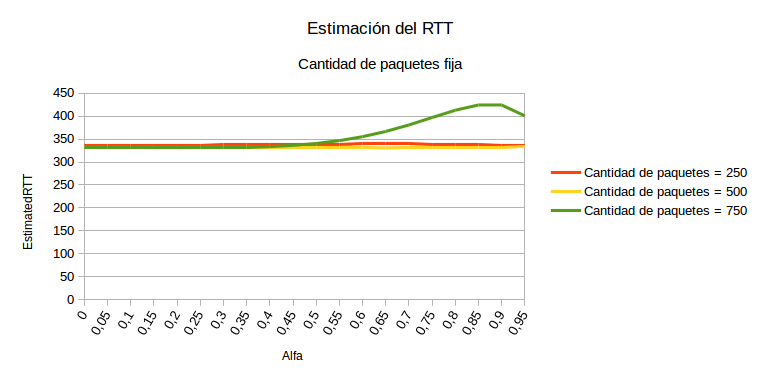
\includegraphics[width=0.8\textwidth]{imagenes/3ra_parte/ping_varios_n_fijo_variando_alfa_rusia.png}}

La gráfica de la Universidad de Tokio es un poco particular, mostrando crecimientos en todas las curvas (en mayor o menor medida) al aumentar el alfa del cálculo de estimaciones. Esto no quita que finalmente los valores tiendan a acercarse a un valor común, representado por el alcanzado en la curva con mayor cantidad de paquetes.

\centerline{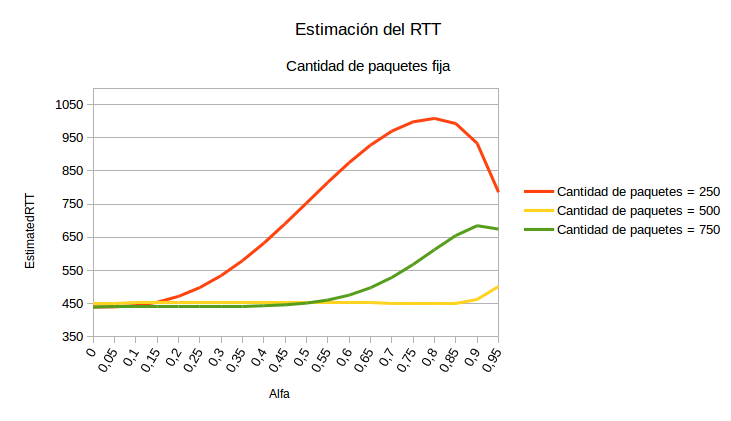
\includegraphics[width=0.8\textwidth]{imagenes/3ra_parte/ping_varios_n_fijo_variando_alfa_japon.png}}

El caso de la Universidad de Boston es el más explícito de todos, revelando como al aumentar por completo el alfa, las estimaciones convergen a un mismo valor, que resulta ser cercano al promedio de las estimaciones parciales.

\centerline{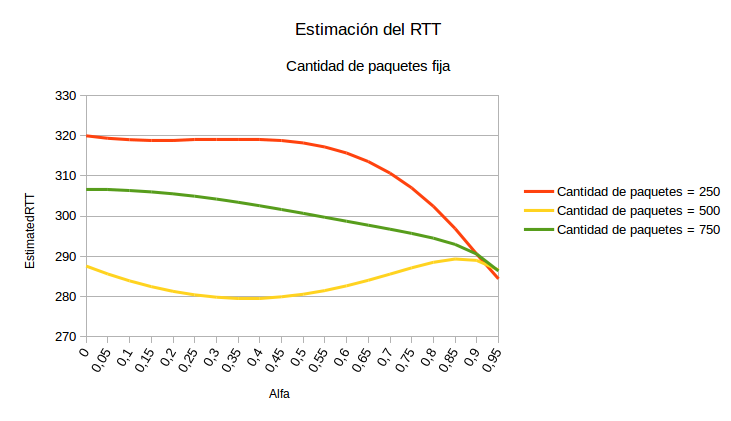
\includegraphics[width=0.8\textwidth]{imagenes/3ra_parte/ping_varios_n_fijo_variando_alfa_eeuu.png}}

\subsection{Estimaciones del RTT}

Teniendo los resultados correspondientes a cada universidad según ambos experimentos, consideramos las estimaciones con mayor valor de alfa (para aquellos con alfa fijo) y el valor promedio al que tienden las curvas (en el caso con cantidad fija de paquetes). La siguiente tabla condensa la información previamente descripta:

\begin{center}
 \begin{tabular}{|c||c|c|c|c|}
    \hline
    Universidad & Berlín & Moscú & Tokio & Boston \\ \hline \hline
    Estimación RTT con alfa fijo & 324,22 & 356,33 & 441,66 & 286,10 \\ \hline
    Estimación con cant. pings fijo & 328 & 354,66 & 655 & 286 \\ \hline
 \end{tabular}
\end{center}

\subsection{Estimación de la probabilidad de pérdida de paquetes}

Al enviar los ping originales a cada una de las universidades con las que estamos trabajando, no sólo habíamos calculado el tiempo insumido (los RTT's), sino que también habíamos contabilizado la cantidad de pings de los cuales no se obtuvo respuesta por parte de cada uno de los hosts. 

Para este experimento, nos dimos cuenta que la cantidad original de pings no era lo suficientemente amplia como para poder apreciar bien la pérdida de paquetes (con 1000 paquetes, hubo ocasiones donde no hubo ninguna pérdida). Por lo tanto incrementamos la cantidad de pings a enviar. Se pasó de mil a diez mil, y se volvió a ejecutar el script.

En base a los datos resultantes, estimaremos entonces cual es la probabilidad de perder un paquete en una conexión con los hosts de dichas instituciones. La fórmula utilizada es la siguiente:

\begin{center}
EstimatedPacketLossProbability = 1 - \frac{#Echo reply}{#Echo request}
\end{center}

En la siguiente tabla resumimos los datos obtenidos:

\begin{center}
 \begin{tabular}{|c||c|c|c|c|}
    \hline
    Universidad & Berlín & Moscú & Tokio & Boston \\ \hline \hline
    #Echo request & 10000 & 10000 & 10000 & 10000 \\ \hline
    #Echo reply & 9984 & #### & 9997 & 9953 \\ \hline
    EstimatedPacketLossProbability & 0,0016 & #### & 0,0003 & 0,0047 \\ \hline
 \end{tabular}
\end{center}

\subsection{Contrastando las estimaciones con resultados previos}

Acá habría que comparar las estimaciones de RTT obtenidas, con los RTT de las consignas anteriores.

\subsection{Simulación del throughput}

Resolver la ecuación de Mantis para cada universidad?

Datos a tener en cuenta:

* MSS: es el Maximum Segment Size. 
Aparentemente MSS = MTU - TCP/IP headers.

Ejemplo encontrado en: alouche.net/blog/2009/09/16/mathis-equation-and-tcp-performance/
MSS = MTU - TCP/IP headers - for example 1460 with an MTU of 1500 (20b IP and 20b TCP headers)

* MTU: es el Maximum Transfer Unit.
https://es.wikipedia.org/wiki/Unidad_máxima_de_transferencia

\begin{center}
BandWidth = \frac{data\ per\ cycle}{time\ per\ cycle} = \frac{MSS * \sqrt{\frac{3}{2}}}{EstimatedRTT * \sqrt{EstimatedPacketLossProbability}}
\end{center}
